\usetikzlibrary{matrix}

\begin{frame}[fragile,label=moveFileDeadlock]{moving two files}
\begin{lstlisting}[language=C++,style=smaller]
struct Dir {
  mutex_t lock; HashMap entries;
};
void MoveFile(Dir *from_dir, Dir *to_dir, string filename) {
  mutex_lock(&from_dir->lock);
  mutex_lock(&to_dir->lock);
    
  Map_put(to_dir->entries, filename, Map_get(from_dir->entries, filename));
  Map_erase(from_dir->entries, filename);

  mutex_unlock(&to_dir->lock);
  mutex_unlock(&from_dir->lock);
}
\end{lstlisting}
Thread 1: \texttt{\scriptsize MoveFile(A, B, "foo")} \\
Thread 2: \texttt{\scriptsize MoveFile(B, A, "bar")} 
\end{frame}

\begin{frame}[fragile,label=moveFileNoDeadlockTimeline1]{moving two files: lucky timeline (1)}
\begin{tikzpicture}
\tikzset{
  timeline/.style={
    tight matrix no line,
    ampersand replacement=\Q,
    nodes={text width=7cm,
      minimum height=0.6cm,
        font=\small\tt\lstset{language=C++,style=small},
        },
    column sep=1cm,
    row 1/.style={nodes={font=\bfseries,align=center}},
    row 2/.style={nodes={font=\bfseries\tt}},
  },
  waiting/.style={text=black!40},
}
\matrix[timeline] (timeline) {
  Thread 1 \Q Thread 2 \\
  MoveFile(A, B, "foo") \Q MoveFile(B, A, "bar") \\
  {lock(\&A->lock);} \\
  {lock(\&B->lock);} \\
  {\normalfont (do move)} \\
  {unlock(\&B->lock);} \\
  {unlock(\&A->lock);} \\
  \Q {lock(\&B->lock);} \\
  \Q {lock(\&A->lock);} \\
  \Q {\normalfont (do move)} \\
  \Q {unlock(\&B->lock);} \\
  \Q {unlock(\&A->lock);} \\
};
\draw[very thick] (timeline-2-1.south west) -- (timeline-2-2.south east);
\end{tikzpicture}
\end{frame}

\begin{frame}[fragile,label=moveFileNoDeadlockTimeline2]{moving two files: lucky timeline (2)}
\begin{tikzpicture}
\tikzset{
  timeline/.style={
    tight matrix no line,
    ampersand replacement=\Q,
    nodes={text width=7cm,
      minimum height=0.6cm,
        font=\small\tt\lstset{language=C++,style=small},
        },
    column sep=1cm,
    row 1/.style={nodes={font=\bfseries,align=center}},
    row 2/.style={nodes={font=\bfseries\tt}},
  },
  waiting/.style={text=black!40},
}
\matrix[timeline] (timeline) {
  Thread 1 \Q Thread 2 \\
  MoveFile(A, B, "foo") \Q MoveFile(B, A, "bar") \\
  {lock(\&A->lock);} \Q \\
  {lock(\&B->lock);} \Q \\
  \Q |[waiting]| {lock(\&B->lock\ldots} \\
  {\normalfont (do move)} \Q |[waiting]|  {\normalfont (waiting for B lock)} \\
  {unlock(\&B->lock);} \\
  \Q {lock(\&B->lock);} \\
  \Q |[waiting]| {lock(\&A->lock\ldots} \\
  {unlock(\&A->lock);} \\
  \Q {lock(\&A->lock);} \\
  \Q {\normalfont (do move)} \\
  \Q {unlock(\&A->lock);} \\
  \Q {unlock(\&B->lock);} \\
};
\draw[very thick] (timeline-2-1.south west) -- (timeline-2-2.south east);
\end{tikzpicture}
\end{frame}

\begin{frame}[fragile,label=moveFileDeadlockTimeline]{moving two files: unlucky timeline}
\begin{tikzpicture}
\tikzset{
  timeline/.style={
    tight matrix no line,
    ampersand replacement=\Q,
    nodes={text width=7cm,
      minimum height=0.6cm,
        font=\small\tt\lstset{language=C++,style=small},
        },
    column sep=1cm,
    row 1/.style={nodes={font=\bfseries,align=center}},
    row 2/.style={nodes={font=\bfseries\tt}},
  },
  waiting/.style={text=black!40},
}
\matrix[timeline] (timeline) {
  Thread 1 \Q Thread 2 \\
  MoveFile(A, B, "foo") \Q MoveFile(B, A, "bar") \\
  {lock(\&A->lock);} \Q \\
  \Q {lock(\&B->lock);} \\
  {lock(\&B->lock\ldots \normalfont{ \myemph{stalled}}} \Q \\
  |[waiting]| \normalfont (waiting for lock on B) \Q {lock(\&A->lock\ldots \normalfont{ \myemph{stalled}}} \\
  |[waiting]| \normalfont (waiting for lock on B) \Q |[waiting]| \normalfont (waiting for lock on A) \\
  ~ \Q ~ \\
  \normalfont{\sout{(do move)}{ }\myemph{unreachable}} \Q \normalfont{\sout{(do move)}{ }\myemph{unreachable}} \\
  \sout{unlock(\&B->lock);}\normalfont{ \myemph{unreachable}} \Q \sout{unlock(\&A->lock);} \normalfont{ \myemph{unreachable}} \\
  \sout{unlock(\&A->lock);}\normalfont{ \myemph{unreachable}} \Q\sout{unlock(\&B->lock);} \normalfont{ \myemph{unreachable}} \\
};
\draw[very thick] (timeline-2-1.south west) -- (timeline-2-2.south east);
\begin{visibleenv}<1|handout:0>
\fill[white] (timeline-5-1.north west) rectangle (timeline.south east);
\end{visibleenv}
\begin{visibleenv}<2|handout:0>
\fill[white] (timeline-8-1.north west) rectangle (timeline.south east);
\end{visibleenv}
\begin{visibleenv}<4->
\node[anchor=north,align=center] at ([yshift=-.5cm]timeline.south) {
Thread 1 holds A lock, waiting for Thread 2 to release B lock \\
Thread 2 holds B lock, waiting for Thread 1 to release A lock 
};
\end{visibleenv}
\end{tikzpicture}
\end{frame}

\usetikzlibrary{arrows.meta,shapes.geometric}
\tikzset{
    >=Latex,
    resource/.style={draw,rectangle,very thick,align=center},
    resource m/.style={draw,rectangle,very thick,align=center,row sep=2mm},
    resource circle/.style={circle,fill=black,inner sep=0mm,minimum width=2.5mm},
    thread/.style={draw,ellipse,very thick,align=center},
    dependency/.style={draw,ultra thick,->},
    dependency future/.style={dependency,dotted},
    dependency reason/.style={align=center},
}

\begin{frame}{moving two files: dependencies}
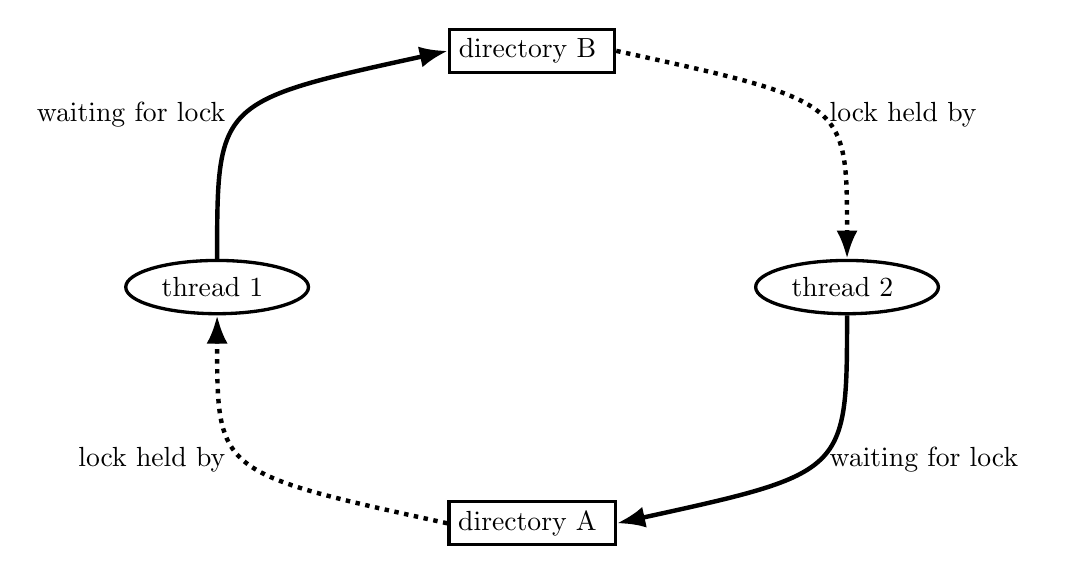
\begin{tikzpicture}
\node[resource] (directory A) {
    directory B 
};
\node[resource] (directory B) at ([yshift=-6cm]directory A) {
    directory A
};
\node[thread] (thread one) at ([xshift=-4cm,yshift=-3cm]directory A) {
  thread 1
};
\node[thread] (thread two) at ([xshift=4cm,yshift=-3cm]directory A) {
  thread 2
};

\path[dependency] (thread one.north) ..  controls ([yshift=2cm]thread one.north) .. (directory A.west)
    node[midway,dependency reason,left] {
      waiting for lock
    };
\path[dependency] (thread two.south) ..  controls ([yshift=-2cm]thread two.south) .. (directory B.east)
    node[midway,dependency reason,right] {
      waiting for lock
    };
\path[dependency future] (directory A.east) .. controls ([yshift=2cm]thread two.north) .. (thread two.north)
    node[midway,dependency reason,right] {
      lock held by
    };
\path[dependency future] (directory B.west) .. controls ([yshift=-2cm]thread one.south) .. (thread one.south)
    node[midway,dependency reason,left] {
      lock held by
    };
\end{tikzpicture}
\end{frame}

\begin{frame}{moving three files: dependencies}
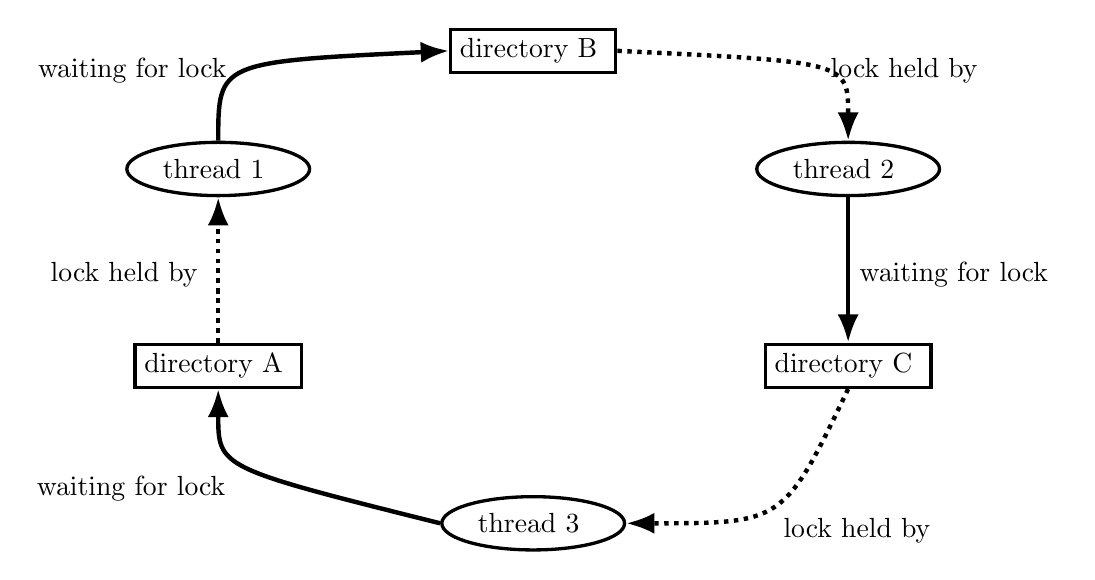
\begin{tikzpicture}
\node[resource] (directory A) {
    directory B 
};
\node[resource] (directory B) at ([yshift=-4cm,xshift=4cm]directory A) {
    directory C
};
\node[resource] (directory C) at ([yshift=-4cm,xshift=-4cm]directory A) {
    directory A
};
\node[thread] (thread one) at ([xshift=-4cm,yshift=-1.5cm]directory A) {
  thread 1
};
\node[thread] (thread two) at ([xshift=4cm,yshift=-1.5cm]directory A) {
  thread 2
};
\node[thread] (thread three) at ([yshift=-6cm]directory A) {
  thread 3
};

\path[dependency] (thread one.north) ..  controls ([yshift=1cm]thread one.north) .. (directory A.west)
    node[midway,dependency reason,left] {
      waiting for lock
    };
\path[dependency] (thread two.south) ..  controls ([yshift=-1cm]thread two.south) .. (directory B.north)
    node[midway,dependency reason,right] {
      waiting for lock
    };
\path[dependency] (thread three.west) ..  controls ([yshift=-1cm]directory C.south) .. (directory C.south)
    node[midway,dependency reason,below left] {
      waiting for lock
    };
\path[dependency future] (directory A.east) .. controls ([yshift=1cm]thread two.north) .. (thread two.north)
    node[midway,dependency reason,right] {
      lock held by
    };
\path[dependency future] (directory B.south) .. controls ([xshift=2cm]thread three.east) .. (thread three.east)
    node[midway,dependency reason,below right] {
      lock held by
    };
\path[dependency future] (directory C.north) .. controls ([yshift=-1cm]thread one.south) .. (thread one.south)
    node[midway,dependency reason,left] {
      lock held by
    };
\end{tikzpicture}
\end{frame}

\begin{frame}[fragile,label=moveFileDeadlockTimeline2]{moving three files: unlucky timeline}
\begin{tikzpicture}
\tikzset{
  timeline/.style={
    tight matrix no line,
    ampersand replacement=\Q,
    nodes={text width=4.5cm,
      minimum height=0.6cm,
        font=\fontsize{9.5}{10.5}\selectfont\tt\lstset{language=C++,style=small},
        },
    column sep=0.25cm,
    row 1/.style={nodes={font=\fontsize{10}{11}\selectfont\bfseries,align=center}},
    row 2/.style={nodes={font=\fontsize{10}{11}\selectfont\bfseries\tt}},
  waiting/.style={text=black!40},
  },
}
\matrix[timeline] (timeline) {
  Thread 1 \Q Thread 2 \Q Thread 3\\
  MoveFile(A, B, "foo") \Q MoveFile(B, C, "bar") \Q MoveFile(C, A, "quux") \\
  {lock(\&A->lock);} \Q ~ \Q ~\\
  \Q {lock(\&B->lock);} \\
  \Q \Q {lock(\&C->lock);} \\
  {lock(\&B->lock\ldots}{ }\normalfont{\myemph{stalled}} \Q \\
  \Q {lock(\&C->lock\ldots}{ }\normalfont{\myemph{stalled}} \\
  \Q \Q {lock(\&A->lock\ldots}{ }\normalfont{\myemph{stalled}} \\
};
\begin{scope}[red!70!black]
\draw[dashed,-Latex,thick,in=-90] ([xshift=-.75cm]timeline-6-1.east) to (timeline-4-2.south);
\draw[dashed,-Latex,thick,in=-90] ([xshift=-.75cm]timeline-7-2.east) to (timeline-5-3.south);
\draw[dashed,-Latex,thick] ([xshift=-.75cm]timeline-8-3.east) to[out=0,in=0] (timeline-3-3.center) to ([xshift=-1cm]timeline-3-1.east);
\end{scope}
\end{tikzpicture}
\end{frame}
